
\renewcommand\chapname{Electronic Grammars and Reproducible Research}	
\renewcommand\longchapname{Electronic Grammars and Reproducible Research}
\renewcommand\shortauthor{Mike Maxwell}
\renewcommand\longauthor{Mike Maxwell\\ CASL/University of Maryland}
\chapter*{\longchapname}
\chapterauthor{\longauthor}
\mytoc{}
 
 
\begin{abstract}
It is time for grammatical descriptions to become reproducible research. In order for this to happen, grammar descriptions must be testable, not only by the original author, but also by other linguists. Given the complexity of natural language grammars, and the ambiguity of prose descriptions, that testing is best done using computational tools to verify a computationally implementable grammar. At the same time, grammars need to be useful---and testable---for the foreseeable future; that is, they must be archivable. Yet if a computational grammar is tied to particular computational tools, it will inevitably become obsolescent. This paper describes a means of creating computationally interpretable grammars which are \textit{not }tied to particular computational tools, nor (to the extent possible) to any particular linguistic theory, and which can therefore be expected to remain useful into the future. In order to make such formal grammars simultaneously understandable to humans, they are embedded into descriptive grammars of a more traditional sort, using the technique of Literate Programming. The implementation of this technology for morphology and phonology is described. It has been used to create morphological grammars for Bangla, Urdu and Pashto which are both human-readable and computationally testable.
\end{abstract}

\section{What can be new about grammars?}


\begin{quote}
An article about computational science in a scientific publication is not the scholarship itself, it is merely advertising of the scholarship. The actual scholarship is the complete software development environment and the complete set of instructions which generated the figures. \citep{BuckheitEtAl1995}
\end{quote}

Of all the methods for documenting and describing languages---the creation of written corpora for linguistic purposes, lexicography, grammatical description, and audio and video collection---it is grammar writing that has the longest history. Grammars of Sanskrit, Tamil, ancient Greek, and Latin date back thousands of years.\footnote{This
 material is based upon work supported, in whole or in part, with funding from the United States Government. Any opinions, findings and conclusions or recommendations expressed in this material are those of the author, and do not necessarily reflect the views of the University of Maryland, College Park and/or any agency or entity of the United States Government.
} 
Oddly, the method for writing grammars has changed little; the invention of glossed interlinear text has been perhaps the most noticeable advance. Even the advent of the computer age, which revolutionized lexicography and corpus creation, and made audio and video documentation practical for the first time, has not significantly changed the nature of grammars. For the most part, grammars continue to be a catalog of the various constructs of the language: noun formation, noun inflection, the order of words in the noun phrase, and so forth, augmented by examples, generally from corpora.  All this could be done just as well on paper as on a computer.

It is true that grammar writing has become easier. Grammar authors can draw from the entire set of characters encoded in Unicode, something which was painfully difficult in the era of typewriters, and often inaccurate when typeset by someone unfamiliar with the language. Modern grammar writers are also blessed with the ability to find examples more easily now that the corpora are on computers; and often these corpora are already stored as interlinear text. Whether the interlinearization has been done consistently has not always been easy to verify, even when the interlinearization was done on computers. But even this is becoming better; SIL's Toolbox has an ``Interlinear Verify'' mode, which flags annotations that don't match lexical entries, and SIL's Fieldworks Language Explorer (FLEx) maintains consistency between the lexicon, grammar, and the interlinear text. Finally, there are now checklists of phenomena to be covered, and often grammars of related languages to draw inspiration from.

While making grammar writing easier is a laudable goal, I believe that a more significant step would be for the resulting grammatical descriptions themselves to change: grammars as language descriptions\footnote{An
  anonymous reviewer has pointed out that there are other sorts of grammars besides rule-based descriptions, including studies of the historical development of grammatical features, typological comparisons, analyses intended to explicate or improve the coverage of a particular theory, and comparative grammatical studies across related languages. In contrast, this paper discusses the grammatical description of a single language, with emphasis on observational adequacy.} must become instances of reproducible research. That is, it must be possible for the reader---indeed, for future generations of linguists---to verify that the grammar is correct, i.e. that it actually describes the language as its author claims. 

One significant step towards this goal has been what I will call ``write-time'' links: links from the examples in the grammar to the location in an electronic corpus from which the author copied them \citep{Nordhoff2008,Thieberger2009}. This allows the reader to view the author's example in context. Indeed, it should be possible to have links to the point in the original audio or video from which the example was transcribed, in principle allowing the grammar user to verify the transcription as well.

Going beyond these author-provided ``write-time'' links to examples, a further step towards reproducible research would be to enable search for grammatical constructions at ``read-time,'' i.e. when the user is reading the grammar. To my knowledge, this innovation has yet to be  implemented. It would require either annotation of a fixed corpus for all the grammatical constructs described in the grammar, or else an on-the-fly grammatical analysis and search facility \citep{Thiebergertv}. The latter method would be superior, since it does not depend on the authors' bias as encoded in the annotated corpus. Furthermore, it would allow searching for grammatical constructions not only over the corpora provided with the grammar, but over any additional corpora that the reader may have access to. 

Several requirements must be met in order to do read-time grammatical search over an arbitrary corpus:

\begin{enumerate}
\item For languages with significant inflectional morphology, there must be a morphological parsing engine. 
\item If the grammar describes syntax, a syntactic parsing engine will also be necessary.
\item The grammar must be represented in a way in which it can be used by the parsing engine(s).
\item There must also be a lexicon compatible with the grammar. Specifically, the grammar and lexicon must use interoperable coding for parts of speech, conjugation or declension classes, etc.
\item A tokenizer must be available, to convert the text into tokens which a parser can deal with. There may also be a need for lower-casing words in scripts that make case distinctions.
\item The corpus must be encoded in the same way as the grammar and lexicon, and use the same writing system (or else it must be possible to convert between encodings and writing systems).
\item Finally, the reader will need a tool which can search through the structures output by the parser.
\end{enumerate}
There are also problems of ambiguity resolution; parsers can be expected to frequently return multiple  parses  \citep[cf][]{Bendertv}. Indeed, even tokenization may be ambiguous.

While ``read time'' search for grammatical constructions is not, to my knowledge, currently possible, I believe it is a desirable goal, for without it the reader is forced to accept at face value the author's description of the language; there is no way to verify the grammar.

This paper describes some steps towards this goal. But first, a discussion of why this goal is important.

\section{Archivable research}
\citet{BirdEtAl2003} drew the attention of linguists to the need for language documentation and descriptions to be archivable. They argued that digital copies of lexicons and texts should be preserved in plain text formats, as opposed to binary formats (such as proprietary database or word processor formats); and in particular, they advocated the use of XML and Unicode. While Bird and Simons said little about how to make grammars archivable, much the same case could be made for descriptive grammars: preservation in XML/Unicode formats is preferable to archiving them in proprietary word processor formats. 

But there is more to be said about grammars. Since at least the 1980s, it has been possible to write grammars in computer-readable format, such that the rules could be turned into a parser and applied to texts. For example, SIL released the AMPLE parsing engine\footnote{I
  make a distinction between a generic {\textit{parsing engine}}, which may be suitable for grammars of a wide range of languages, and a {\textit{parser}}, which is the application of a parsing engine to a particular language. Parsers are usually built from three parts: the generic parsing engine, a language-specific grammar in a format readable by the parsing engine, and a language-specific dictionary, also in a format readable by the parsing engine.
}
\citep{WeberEtAl1988}, which has subsequently been used to create morphological parsers for many minority languages; other morphological and syntactic parsing engines have become available since then. Bird and Simons did not touch on how (or whether) computer-readable grammar rules for such parsers should be preserved. However, \citet{AmithEtAl2005}, \citet{MaxwellEtAl2005} and \citet{MaxwellEtAl2008} discuss the following problem: while we can preserve the grammar rules that could be used by this or that parsing engine, the parsing engines themselves---like any software---will eventually become obsolete. The question then is how computer-readable grammar rules, suitable for parsing corpora, can be archived. In particular, how can we write grammars incorporating such rules in a way that the grammars will be usable long after the original parsing engine has become obsolete?

The work presented here builds on these issues of archivability, but expands on them by considering how making a grammar including computer-interpretable rules archivable also contributes to making such a grammar an instance of reproducible research. I now turn to that issue.

\section{Reproducible research}
\begin{quote}
  Abandoning the habit of secrecy in favor of process transparency and peer review was the crucial step by which alchemy became chemistry \citep{Raymond2004}.
\end{quote}

A fundamental requirement of modern scientific research is that the results be reproducible. This can of course mean different things in different sciences; for medical research, it generally means that the application of a treatment to a different group of patients will lead to similar statistical results. But in sciences like astronomy, where an event like a nearby supernova may not be repeated for centuries, it means being able to reproduce analyses from an archived set of data. Language description has elements of both of these kinds of research. For many languages, it is possible to collect additional data, which may be used as additional test cases to confirm or refute a grammatical analysis. But it may be difficult to collect new data from ``exotic'' languages, and impossible with extinct languages, so that reproducibility in such cases means being able to verify that the structures of a fixed corpus can be generated from a lexicon and rules. 

In a sense, linguistics has long been about reproducible research. Grammars have included examples, often in the form of interlinear text, presumably intended not only to illustrate the abstract grammar rules, but also to allow the reader to verify the rules. In some cases, text corpora are published together with the grammar; recently, \citet{BahraniEtAl2011} included a small corpus of test sentences they used to evaluate their syntactic parser. But therein lies the problem: while it may be possible to verify a rule, or a small set of rules, on a few cases, verifying all the rules on all the examples of the grammar, or worse on an entire corpus, is beyond the patience or even ability of most of us. Languages and their grammars are simply too complex; and as a result, research in linguistics is all too often not verifiable in practice. Indeed, with rare exceptions (such as D. Payne's 1981 grammar of Axininca Campa), published grammars are not explicit enough to support verification. \nocite{Payne1981}

In addition to the fact that grammars are often too difficult to test by hand, two other factors make it virtually impossible for traditional descriptive grammars to constitute reproducible research. First, even the best of grammars generally have gaps in coverage. This is of course true for syntactic grammars, but it is also true for morphological grammars of languages with complex morphology. As \citet{Bauer2010} writes, 
\begin{quote}
 reliance on grammars is not sufficient to give completely accurate data... Descriptive grammars rarely exemplify derivational patterns in any detail, rarely say what is productive and what is not, rarely tell you whether the examples they provide are regular or not, and typically provide lexicalised examples. In other words they do not usually provide precisely the kind of information that the morphologist would like to know about.
\end{quote}

Second, the fact that descriptive grammars are themselves written in ordinary languages such as English means that they are inevitably ambiguous. The problem of ambiguity has been discussed for decades in the context of writing specifications for computer programs; see e.g. \citet{Abbott1983}, \citet{Wiegers2003}, \citet{Meyer1985},  \citet{BerryEtAL2003}, and \citet{KamstiesEtAl2003}. The situation is no different, in my experience, for grammar writing; grammatical descriptions are unclear and ambiguous in unforeseen and probably unforeseeable ways. Experience by our team of grammarians at the University of Maryland has found many examples of unclear writing, even in the best of grammars, resulting in our needing to determine what is really going on in the language by consulting other grammars, talking with other linguists working on the languages, and doing our own fieldwork and corpus research. These problems will not go away by trying to write more clearly. The fact that natural language is not sufficiently clear and unambiguous is one of the reasons that natural languages are not, despite years of trying, used for programming computers. Rather, making grammar writing truly reproducible requires that we have an unambiguous way of expressing grammar rules and constraints: a formal grammar, analogous to a computer programming language. 

For these same reasons,  in many scientific fields the term ``reproducible research'' has come to mean something like the following :

\begin{enumerate}
\item Publication of an analysis in more or less the usual form, such as an article in a journal or conference proceedings.
\item Publication of the data used in the analysis in downloadable form.
\item Publication of the software used to perform the analysis in downloadable form. 
\end{enumerate}

This form of reproducible research thus differs from simply data archiving in that not only the data, but the software used for analysis, is made available to other researchers. The analysis described in natural language provides an easily read view of what the authors did, but the published software and data provide the final complete and unambiguous description with which their claims can be verified.

Reproducible research of this sort is often documented by using Literate Programming \citep{Knuth1992} to produce a ``compendium,'' a computer-readable version of the document combining a textual description for human consumption with the software program for computer consumption \citep{GentlemanEtAl2004}; that is, parts (1) and (3) above, and sometimes the data (part 2). This compendium can be obtained by other researchers, who can extract software for verification against data, whether data contained in the compendium, or other relevant data.

In the Literate Programming paradigm, the ordinary published paper (item (1) in the above list) can be produced as a readable ``view'' of this compendium document, by an automatic conversion process.  In fact, it is possible to produce multiple print views from the same compendium; a standard print view might include the program code used to analyze the data, while a view for publication in a conference proceedings might omit this code because of page limitations.

Literate Programming has been used to publish reproducible research in geophysics \citep{ClaerboutEtAl1992}, bioinformatics \citep{GentlemanEtAl2004,Hothorn2011}, epidemiology \citep{PengEtAl2006}, signal processing \citep{BuckheitEtAl1995,VandewalleEtAl2009}, statistics \citep{Leisch2002,DonohoEtAl2009,LenthEtAl2011}, econometrics \citep{KoenkerEtAl2009}, and other fields.

Moving in this direction, as of 2011 National Science Foundation grant proposals must include a data management plan (\url{http://www.nsf.gov/pubs/policydocs/pappguide/nsf11001/gpg\_2.jsp\#dmp}). While this addresses the availability of the data leading to an analysis, it does not attain the full goal of reproducible research. Specifically, it does not require publishing the computational methods used to process the data. Some journals have accordingly gone further, encouraging authors to submit their articles as true reproducible research using Literate Programming: 
the {\textit{Annals of Internal Medicine}} \citep{LaineEtAl2007};
{\textit{Biostatistics}} \citep{Peng2009};
{\textit{The Insight Journal}} (see \url{http://www.insight-journal.org/});
{\textit{Computing in Science and Engineering}} \citep{FomelEtAl2009}; and 
{\textit{IEEE Transactions on Signal Processing}} (see \url{http://www.signalprocessingsociety.org/publications/periodicals/tsp/}).
The publisher Elsevier has sponsored the ``Executable Paper Grand Challenge'' at the The International Conference on Computational Science in Singapore in June 2011. For linguistics, the new {\textit{Journal of Experimental Linguistics}} (\url{http://www.elanguage.net/journals/index.php/jel/index}), part of the LSA's eLanguage initiative, could begin to address these issues.

At the University of Maryland, we have begun using Literate Programming to document grammars of natural languages, particularly the morphology and phonology of these languages, as reproducible research. As with other Literate Programming approaches, our grammars consist of two interwoven parts: one is a traditional descriptive grammar, complete with interlinear examples; the other, a formal grammar, is intended for use together with a lexicon as a morphological parser. Our approach differs from that of most previous work in Literate Programming in that our formal grammar is not written in the programming language of some existing piece of software. Rather, our formal grammar is a structured XML description of the grammar. Creating a parser in order to verify the grammar against a set of examples or a corpus thus requires an additional step: converting the XML description into the programming language of a suitable parsing engine. We have added this step because of the importance in linguistics of archivability: it safeguards our formal grammar against the inevitable obsolescence of the parsing engine, a point to which we return later in this paper.

\section{Producible research}
\begin{quote}
 The tale of the Zigglebottom Tagger is one of disappointment, not just for you but also for Zigglebottom himself. While his work achieved publication, it must gnaw at his scientific conscience that he can't reproduce his own results \citep{Pedersen2008}.
\end{quote}

For the reasons outlined above, I believe reproducible results should be a clear requirement in the field of linguistics, and for grammar descriptions in particular. But before a result can be reproducible, it must be producible---that is, it must be possible for the researchers to verify their own results. Sadly, that is not true of many grammars. When a grammar has any significant degree of complexity, it is too difficult and time-consuming to test every grammar rule on every form in a corpus, keeping in mind every constraint on rule application provided by the theory. Instead, grammar writers generally test their rules (or perhaps only the rules which they expect to be relevant) to selected test cases.

This happens for rule-based grammars (which are the focus of this paper), but the problem is at least as bad with constraint-based systems like OT: there are too many active constraints, and too many possible forms (infinitely many, in most OT theories) to determine the correct answer by hand in any but a small set of test cases. Lauri Karttunen makes this point clearly, speaking of OT: ``Paper-and-pencil methods are insufficient to test a theory with real data'' (2006: 287). \nocite{Karttunen2006}

This is not to say that there are not grammars which are relatively simple, and which could therefore be tested by hand. The inflectional morphology of English, for example, is not hard to test; and purely agglutinating morphologies, with little or no allomorphy, are often testable by hand. But when significant morphology interacts with significant phonology to create significant allomorphy, it is all too easy to overlook rule interactions, with the probable result that not all forms in the corpus can in fact be derived by the proposed grammar. Syntax is, of course, still more complex, and it is correspondingly more difficult to determine whether a syntactic grammar accounts for a corpus.

As \citet{Pedersen2008} suggests with his tongue-in-cheek description of the ``Zigglebottom Tagger'' quoted above, failure of other researchers to reproduce published results may cause the author to question whether the results were correct in the first place. The methodology described in this paper thus provides a way for other linguists to not only reproduce, and thereby verify, grammatical descriptions, but for the author to validate the grammar in the first place, in as much detail, and with as many test cases as desired.

Some readers may be asking whether the problem is really as bad as I am painting it. Surely most grammars are explicit enough that the authors, at least, have validated them, and that other linguists could in principle validate them? It is impractical to answer this for all grammars, so I will instead supply some examples from my personal experiences in grammar writing.

I first encountered the difficulty of telling whether my own grammatical analysis covered the data  when I co-authored a grammar of Cubeo, an agglutinating Tucanoan language \citep{MorseEtAl1999}. The difficulties in verifying the analysis had to do with both morphology and syntax. I could check a few example sentences for conformance to the generalizations my co-author and I made, but it was beyond us to check all the examples for conformance to all the grammar rules. Indeed, after the published grammar appeared, I realized that my analysis failed to correctly generate some of the cells in the verb paradigm. I am afraid to find out what other errors might surface if I wrote a Cubeo parser and tested it against a corpus, or even against the examples in the book.

My suspicion of how hard it was to verify a grammar against a corpus was confirmed a few years later, when I worked with Jonathan Amith on the Oapan dialect of Nahuatl. My task was to write a morphological parser, using the Xerox finite state toolkit (\texttt{xfst}, see \citet{BeesleyEtAl2003}). This dialect of Nahuatl combines the polysynthetic nature of all varieties of Nahuatl with a particularly messy set of phonological processes. Our analysis has more than 30 rules to derive verb stem allomorphs, which interact in complex ways with aspectual marking and with lexically defined allomorphy classes, plus another 30-odd general phonological rules; many of these rules are crucially ordered with respect to each other. This last problem---that of determining rule ordering---was particularly problematic, as it was not always obvious whether two rules could interact, and crucial cases often did not appear until months after we had written the two rules. When we encountered an erroneous form, we had to debug the grammar in order to discover where the error came from: it might be because we had written one of the rules incorrectly, or because the rules were incorrectly ordered.\footnote{We
  might also have chosen the wrong underlying form of a morpheme; but  that seems to have been less of a problem in our case.} The cause was almost never apparent from inspection, and the only way to discover it was to temporarily remove rules which might be interfering, or to modify rules, or to re-order the rules until the correct form was produced. Occasionally it was necessary to inspect intermediate forms. It would have been helpful to automatically produce a trace of the rule application (a derivation), although that happens not to be straightforward in the \texttt{xfst} tool. While this may seem bad enough, it was not always the case that our first repair was right: sometimes fixing the rule for one form would cause other previously correct analyses to fail. 

Almost none of these problems could be found by inspection; we only knew about them when we ran the parser over all our test data and compared the results with previous results, to look for unanticipated changes.\footnote{In
  software development, this is called ``regression testing,'' and it is supported by an array of tools, including version control systems and `diff' (for ``difference'') tools. The writing of linguistically motivated computational grammars is highly dependent on such software development tools.
}
Even when we knew there was a problem, it was often unclear what rule or rules caused the problem, how to fix it, or what the implications of a fix would be across the grammar and lexicon. In summary, it was generally impossible to tell by inspection whether an analysis covered all the data in the corpus.

It is important to say that these problems in converting a descriptive grammar into a parser do not constitute a criticism of Amith's grammar writing ability (or, I hope, of my ability to understand descriptive grammars). Rather, this need for clarification, disambiguation and testing happens whenever humans write complex descriptions. In summary, the capability of building a parser based on one's grammar and a lexicon, and testing this against the examples of the grammar and against a corpus, is the only way to verify that one's own grammar works.

Having discussed the problems of making grammatical analysis archivable, reproducible and  producible, I now turn to our solution, consisting of three parts: a descriptive grammar, a formal grammar, and a way of testing the grammar against real data.

\newpage
\section{Descriptive grammar}
\begin{quote} 
 Literate programming has many adherents, but it failed to become mainstream programming technology.  Partly, we believe, this is due to many programmers' aversion to writing documentation in any form.  But we in the mechanical theorem proving community do not have the luxury of avoiding documentation. For one thing, proofs are often much more complex than programs; many of us prove theorems about programs. \citep{Gamboa2003}
\end{quote}

Like researchers in theorem proving, linguists have a long history of documenting the grammars of languages: traditional descriptive grammars are entirely documentation, and the descriptive grammars we have been writing at the University of Maryland are not much different. In order to make them more likely to be useable in the long run, and therefore meet the needs of archiving, in our grammar writing we avoid binary formats and instead use a well-documented XML-based standard, DocBook \citep{WalshEtAl2011}. DocBook was designed for technical documentation, particularly computer documentation. As such, its schema (the configuration document that describes what a valid DocBook document is) has provision for many constructs which are needed to describe software, but which are irrelevant to language description. While these may be simply ignored, it is easy enough to customize the schema to omit the unneeded constructs, thereby ensuring that they are not inserted accidentally.\footnote{There
  is a project to produce a simplified DocBook (\url{http://www.docbook.org/schemas/simplified}), omitting many of these specialized constructs. However, as I write this, it is only available in a DTD form, which was used with DocBook version 4; DocBook version 5, which we are using, uses a RelaxNG schema (see \url{http://www.relaxng.org/}). The DocBook organization is working on a simplified schema corresponding to version 5, which may be published by the time this paper reaches press. The DocBook Publishers Schema (\url{http://docs.oasis-open.org/docbook/specs/publishers-1.0-spec-cd-01.html}) is similar in intent to Simplified DocBook, and uses a RelaxNG schema. Our modified schema is substantially similar to the DocBook Publishers Schema, modulo the additions we have made for linguistic data.}

As an alternative to DocBook, we could have used some subset of the TEI document encoding (\url{http://www.tei-c.org/Guidelines/P5/}). We have no strong opinions on the merits of DocBook vs. TEI; our decision was based on familiarity with DocBook, and the availability of tools that made it easier to use. Porting descriptive grammars from DocBook to the TEI format should not be difficult.\footnote{Another
  alternative for the descriptive grammar might be the NLM (National Laboratory of Medicine) ``NCBI Book Tag Set'', see \url{http://dtd.nlm.nih.gov/book/}.
}

Descriptive grammars typically make use of a few specialized constructs, such as interlinear text. We have therefore enriched the DocBook schema to allow not only for glossed interlinear examples,\footnote{Our
  XML schema for interlinear text and the style sheet for displaying it were simplified from code made available by Andy Black, of SIL, which he had developed for his own grammar documentation project. See also \citet{HughesEtAL2003} for a general model of interlinear text.
} 
but also for inline examples. The latter are one or two word examples, typically in the main text or in paradigm tables. Because we tag interlinear and inline examples as XML elements, they can be automatically extracted as test cases for the parser. This is an essential aspect of ensuring that our grammars are reproducible. If we relied on a traditional corpus alone for parser testing, we could not ensure that the parser covered all paradigm cells in all paradigm classes, because the corpus might lack rare forms, such as vocatives. But if we have sample paradigms for all declensions or conjugations, stem allomorph classes,\footnote{Our
  grammatical formalism distinguishes inflection (declension and conjugation) classes, which refer to the choice of affixes, from stem allomorphy classes. Since stem allomorph classes often cross-cut inflection classes, this represents a useful partitioning of information. There are also theoretical reasons for distinguishing the two notions, see e.g. \citet{Carstairs1987}, particularly chapter 6.
} 
and irregular (suppletive) words, then we ensure that we have at least one test case for each paradigm cell of every word class.

While we could simply embed the formal grammar as an appendix to the descriptive grammar, we have followed the usual practice in Literate Programming by breaking the computer-readable program{ (}in our case, the formal grammar described below{) }into ``fragments,'' and placing these fragments in the relevant places throughout the descriptive grammar. For example, the formal grammar fragment for the affixes of the first noun declension class in Pashto appears in the section of the descriptive grammar describing this class. Supporting this capability required augmenting DocBook by the addition of a couple of elements (modified from \citet{Walsh2002}): one to enclose the fragments of our formal grammar in the descriptive grammar, and one to provide a mechanism to re-unite those fragments in the correct order as a single file suitable for conversion to a parser. (This process of re-uniting the fragments is discussed in the next section.)

In order to produce a typeset grammar from our XML grammar, it is necessary to convert the XML document into some other form. DocBook documents are commonly typeset by conversion to ``XSL-FO'' (XSL Formatting Object) format, although they can also be converted to Microsoft Word. However, our experience with conversion to Word showed that manual post-editing was necessary, and the need for rapid turn-around (e.g. to make changes near the end of grammar writing) made that impractical. The XSL-FO route did not appear to produce sufficient quality for our multi-lingual work, particularly where non-roman scripts were involved---and all our grammar work thus far has included non-roman scripts (the Bengali script, the Nastaʿliq style of the Arabic script for Urdu and Punjabi, the Naskh form of the Arabic script for Pashto, and soon the Thaana script for Dhivehi). Fortunately, two pieces of the puzzle came together at the right time to solve our problem. Jonathan Kew created the XeTeX program (\url{http://scripts.sil.org/xetex}), a Unicode-aware version of the excellent LaTeX typesetting program; and Benoît Guillon created the dblatex program (\url{http://dblatex.sourceforge.net/}), allowing for conversion of DocBook documents to LaTeX format. Since dblatex is distributed as open source, modifying it to convert our added constructs was not difficult; and LaTeX (and therefore XeTeX\footnote{Almost
  all LaTeX packages are usable with XeTeX, and the user community has been most helpful. Most recently, Apostolos Syropoulos modified a package enabling the use of change bars so that it worked in XeTeX---for free!
}) 
already has packages for typesetting interlinear text, as well as a host of other useful packages. Together, these pieces of software allow us to produce high quality PDFs of book-sized grammars in a matter of minutes, with no manual intervention.\footnote{Software
  to convert DocBook documents into HTML form is also available.
}

We also wanted to be able to produce PDFs of our grammars for diverse audiences. For example, someone interested only in using our grammar as a desk reference might not wish to see the formal grammar, but might want explanations of linguistic terms that would be superfluous to a linguist. Also, we occasionally add descriptions of alternative grammatical analyses, such as an explanation for why we chose a particular set of declension classes to describe Pashto (published descriptions of Pashto range from five declension classes to a dozen); these explanations would be of little interest to most non-linguists. For this purpose, DocBook provides an attribute called ``audience.'' For our work, we set this to ``tech'' on portions of text that we want to hide from a non-technical audience, or ``non-tech'' for pieces of text to be hidden from a technical audience (and we leave the attribute unmarked on text that is appropriate for both audiences). When we create the PDF, we tell the conversion process to omit the non-relevant portions, giving us output tailored for the particular audience.\footnote{Obviously
  we could make finer distinctions than ``tech'' vs. ``non-tech'' if we wished \citep{Barabytv}
}

\section{Formal grammar}
\begin{quote}
 I thought the specifications were precise, but nobody understands how imprecise a specification is until they try to explain it to a computer. And to write the program. \citep[608]{Knuth1996}
\end{quote}

Unlike descriptive grammars, the notion of a formal grammar of the sort we are using is relatively new. Our formal grammar is intended to represent much the same information as that conveyed by the descriptive grammar, but in a form that is computer readable---specifically, in a form that can be converted into a parser without human intervention. We had several desiderata for this grammar representation formalism:

\begin{enumerate}
\item The formalism should cover a wide range of linguistic constructs.
\item It must be suitable for a typologically wide variety of languages.
\item While designed to be computer-interpretable, it must also be human readable with a modicum of training.\footnote{In
  this respect, the grammar formalism resembles a high level programming language such as Python.
}
\item It should be, to the extent possible, self-documenting. That is, each piece of language-specific information should be tagged for its function using mnemonic tags.
\item The linguistic theory behind the formalism should be understandable a decade or a century from now.
\item The formalism should work together with other formalisms used for language documentation and description. 
\end{enumerate}

The XML-based formalism we developed largely meets the above desiderata, as described below.

\subsection{Coverage of linguistic constructs}
Our formalism covers most morphological and phonological constructs. It does not cover syntax, semantics, or pragmatics; but coverage of morphology and phonology, without syntax, is adequate for the creation of morphological parsers. Indeed, interlinear text glossing typically (and not coincidentally) is done using exactly the same range of markup as our formal grammar covers: very rarely does interlinear text markup include syntactic annotation. 

Some linguistic objects such as lexicons are already covered by other standards, and the formalism described here is intended to work with those standards, not duplicate them, as described in section 6.6.

Within morphology, the coverage of the formalism includes the following:

\begin{itemize}
\item Inflectional and derivational morphology
\item Morphosyntactic features
\item Exception features (e.g. for stem allomorph classes)
\item Prefixes, suffixes, infixes
\item Reduplication and other sorts of process affixes
\item Position classes for inflectional affixes (inflection can also be modeled without such classes)
\item Inflection classes (conjugation and declension classes) 
\item Compounding, incorporation
\item Listed phonologically conditioned allomorphs (for roots, stems, and affixes)
\item Listed irregular (suppletive) word forms
\end{itemize}
In the domain of phonology, the coverage includes the following:

\begin{itemize}
\item Phonemes, graphemes, and boundary markers
\item Natural (or unnatural) classes, defined as sets of phonemes
\item Phonological rules, including epenthesis and deletion rules
\end{itemize}

\begin{itemize}
\item Rules apply in linear sequence.
\item Rule strata can be defined.
\item Rules can apply simultaneously, or iteratively left-to-right or right-to-left.
\item Environments are definable as regular expressions over phonemes, graphemes, boundary markers, natural classes, and strings.
\item Phonological rules can be restricted to a particular part of speech.
\item Rules can require the presence or absence of an exception feature.
\end{itemize}

Notice that phonologically conditioned allomorphy can be treated by either listing the allomorphs and their conditioning environments, or by deriving allomorphs from underlying forms using phonological rules. The former is often easier to use for affixes, and indispensable for suppletive allomorphs, while treatment by rule is often easier for stem allomorphy.

As of now, most of the above constructs can be converted for use by the parser; see section 7. 

\subsection{Applicability to typologically diverse languages}
Initial development of the grammar formalism was done around 2000 under the auspices of SIL International, and in particular with the help of Gary Simons and Andy Black, both members of SIL. The concern was to ensure that to the extent possible, the formalism supported accounts of the morphology and phonology of the world's languages at the observational level of adequacy (in the sense of \citet{Chomsky1965}; see further in section 6.5). Much of this work involved searching through publications to ensure that the model we were building covered the sorts of constructions described there. For the most part, these publications were theoretical works on morphology and phonology, particularly handbooks of morphology and phonology, since these served in effect as a distillation of published grammars. The resulting catalog of construction types outlined in the previous section is, we are confident, adequate to cover most of the morphological and phonological constructions found in the grammars of individual languages. However, some limitations will be described below. In particular, over- and under-application of phonological rules in reduplication may be difficult or impossible to describe in this formalism. Also, some linguists may consider the coverage of syllabification and stress assignment to be inadequate.

\subsection{Computer interpretability vs. human understandability}
The focus of this paper is on documenting grammars, not on how those grammars are created. Our formal grammars are, at least for now, written by humans; it may become possible to automatically adapt a formal grammar from one language to a closely related language, or to induce formal grammars from bitext, particularly from existing interlinear text (see \citet{LewisEtAl2008} for some ideas along these lines). But regardless of how the grammars are created, we take it as important that they be understandable by humans. At the same time, if the formal grammar is to used to build a parser, then  like any programming language it be must be interpretable by the computer without human help.

Furthermore, as words are found which fail to parse (generally by building a parser from the formal grammar and discovering where it fails), it must be possible to find the cause of the problem. Errors can occur in any of several places: the original corpus may be in error (someone may have mistyped a word, for example); the lexicon may have an error, or be missing a word;\footnote{Frequently
  these are proper names or loan words.
}
or the grammar may have an error. Discovering such errors goes beyond the scope of this article; suffice to say that building parser debugging tools is another area needing attention.

Ultimately, such problems must be fixed, and when the error turns out to be in the grammar, it must be possible for the human to understand that grammar. One method that is often used in ordinary computer programming is to embed comments in the program code, which can be ignored by the computer. It is an oft-lamented fact that computer programmers frequently fail to comment their code, or comment it inadequately. As it happens, linguists have---if anything---the opposite problem: a traditional descriptive grammar is all comments, and no code! The grammar writing framework we are advocating here has both comments---the descriptive grammar---and code---the formal grammar. Moreover, because the formal grammar is scattered in the form of fragments throughout the descriptive grammar, each fragment is explained by the nearby text, and exemplified by the nearby examples. This obviously contributes to the human understandability of the formal grammar, and therefore to a human's ability to debug it. This is not to say that it the intent of each statement in the formal grammar is likely to be immediately obvious, but our mingling of the formal and descriptive elements of the grammar certainly makes the reader's learning curve for the notation less of an impediment.

\subsection{Self-documenting}
Linguists have long used formal conventions for linguistic constructs. For example, in the past phonological rules were often written like either of the following:

\ea  $\left\{
       \begin{array}{l}
             b\\
             d\\
             g
        \end{array}
        \right\}
   \rightarrow 
       \left\{
       \begin{array}{l}
           p\\
           t\\
           k
        \end{array}
        \right\}
    {\mathrm{/}}\mathrm{\_\_\#}$
\z

\ea  $\left[
      \begin{array}{l}
           -\mathit{sonorant}\\
           -\mathit{continuant}
      \end{array}
      \right]
    \rightarrow 
      [-\mathit{voiced}]\mathrm{/\_\_\#}$
\z

The curly braces in (1) represent an ordered list of alternatives, implicitly matched between the two braced sets (`b' corresponds to `p', `d' to `t', and `g' to `k'), while the square braces in (2) represent an unordered set, both elements of which must be true (a phoneme to which this rule applies must be simultaneously non-sonorant and non-continuant). In both cases `\#' is represents a word boundary. While the meaning is probably clear to most linguists today, the reliance on arbitrary characters is troubling from the perspective of long-term understandability. Will a reader a hundred years from now understand these notations, or notations for rules of epenthesis, deletion, reduplication etc.? And does the rule apply simultaneously, left-to-right iteratively, or right-to-left iteratively? Both notations are silent on this latter question.

In order to avoid this issue of ambiguous or non-readily understood notations, our formal grammars use explicit labels on all linguistic constructs, in the form of XML tags. An example is the following, encoding rule (1) above:\footnote{Each
  of the XML tag names in this example is preceded by a ``namespace'' prefix, here ``\texttt{Ln}'', distinguishing them from standard DocBook tags; this namespace also identifies the version of the XML schema to which the formal grammar tags belong. The implication is that if the schema is changed later, to correct some deficiency or add a new construct, the correct version of the schema will still be unambiguously identifiable. Also, a few comments in the example are enclosed in the XML comment format, using ``\texttt{{\textless}!---}'' before and ``\texttt{---{\textgreater}}'' after.
}
\ea
\begin{verbatim}
  <Ln:PhonologicalRule direction="simultaneous">
    <Ln:subrules>
      <Ln:PhonologicalSubrule>
        <!--- b -> p --->
    <Ln:input><Ln:refPhoneme idref="b"/></Ln:input>
        <Ln:output><Ln:refPhoneme idref="p"/></Ln:output>
      </Ln:PhonologicalSubrule>
      <Ln:PhonologicalSubrule>
        <!--- d -> t --->
        <Ln:input><Ln:refPhoneme idref="d"/></Ln:input>
        <Ln:output><Ln:refPhoneme idref="t"/></Ln:output>
      </Ln:PhonologicalSubrule>
      <Ln:PhonologicalSubrule>
        <!--- g -> k --->
        <Ln:input><Ln:refPhoneme idref="g"/></Ln:input>
        <Ln:output><Ln:refPhoneme idref="k"/></Ln:output>
      </Ln:PhonologicalSubrule>
    </Ln:subrules>
    <Ln:environments>
      <Ln:Environment wordFinal="true"/>
    </Ln:environments>
  </Ln:PhonologicalRule>
\end{verbatim}
\z

While this notation might seem cumbersome, it has the virtue of being unambiguous: the fact that `b' corresponds to `p', `d' to `t', and `g' to `k', which was implicit in rule (1), is now made explicit.\footnote{The
  individual phonemes to which the rule applies are encoded elsewhere,in the formal grammar, as a part of the phoneme inventory (or alternatively, a grapheme inventory) of the language. The input and output of the rule therefore refer to those phonemes defined elsewhere by means of an XML \texttt{``idref}''. The idref can be any string; in practice, we usually use longer names than are shown in the example, like \texttt{`phG}' for the phoneme `g'.
} 
Moreover, the use of an arbitrary character (`\#') to represent the fact that the rule applies word-finally is now represented by an explicit attribute (\texttt{'wordFinal'}). And lastly, the function of each part of the rule is given by mnemonic XML tag names like `\texttt{Environment}', rather than by arbitrary characters (the slash on the left of rule (1), and the end of the line on the right). 

At present, the formal grammar is written as raw XML using a programmer's editor, which provides support for open- and close-tag matching, syntax-directed coloring, schema validation, etc. We intend to build support for a structured editor for the formal grammar, analogous to the DocBook editor we are using for the descriptive grammar; we believe this would make the grammar writer's learning curve  much easier.\footnote{For
  now, we use either jEdit or emacs, although there are other programmer's editors that would work as well. XML-specific editors such as Oxygen and XMLmind also exist; what we have not yet developed for those editors is a Cascading Style Sheet (CSS) that would enable on-screen formatting, in place of the raw XML tags.
}

This XML notation can, in principle, be typeset in a simpler format, such as that of rule (1) above. Notice that the process of typesetting does not change the underlying XML representation, which remains unambiguous and self-documenting, and therefore suitable for long-term archiving. We have not yet written the program to convert the formal grammar from the XML into a typeset format like (1), but it would use mechanism similar to that used to produce the typeset DocBook XML.

\subsection{Linguistic theory behind the formalism}
\label{bkm:RefHeading72467100141}
The reader may wonder why the formal grammar fragment in (3) uses phonemes, rather than phonological features. This may seem particularly odd in view of the earlier discussion of the need for broad typological and linguistic coverage. In fact, most of the machinery which the formalism makes available would be comprehensible, if not already familiar, to an American structuralist from the 1950s. This is a conscious decision, motivated by several factors.

First, linguistic theories are diverse, and change frequently. If we chose to model one of the latest theories, we would risk making it usable by only the current practitioners of that model---losing both present and future linguists who might prefer a different theory. Instead, we choose to model grammars using a theory which is long past its popularity, but which is stable and relatively easy to understand;  paradoxically, we believe this allows its use by linguists of many different theoretical persuasions. 

For example, the fact that we do not use phonological features renders arguments over feature underspecification irrelevant. This not only means that we do not need to take a stand on this issue, but that a linguist using our system for practical work does not need to worry about which theory of the application of phonological rules to underspecified representations we have used---our representations consist of phonemes, boundary markers and the like, all of which are either present or not.

Moreover, the use of a theory which is in large part fifty years dead means that most of the problems with it have been worked out. And as it turns out, most of those problems are either solvable by the addition of a few ideas from later eras (such as ordered phonological rules), or have no effect on observational adequacy. Before turning to the additions we have made to what would otherwise be a 1950s-era linguistic model, I will clarify why we are content with observational adequacy.

\citet{Chomsky1964,Chomsky1965} introduced three levels of linguistic adequacy: observational, descriptive, and explanatory. A grammar which met the {\textit{observational level of adequacy}}  would be capable of generating all and only the sentences of the language---or, if one's interests were confined to morphology and phonology, all and only the possible word forms of the language. 

A {\textit{descriptively adequate}} grammar would go further, to account for intuitions that native speakers have. For example, a descriptively adequate grammar of English syntax might provide structural descriptions which would allow for disambiguating the two meanings of sentences like ``The chicken is ready to eat.'' In phonology, it has been argued \citep{ChomskyEtAl1965} that the intuition by native speakers of English that the non-word {\textit{blick}} would be a more acceptable English word than the non-word {\textit{bnick}} is due to the internal phonological grammar that English speakers have, and that a descriptively adequate phonology of English should account for this.  

Finally, a linguistic theory (as opposed to a grammar) is said to attain to the {\textit{explanatory level}} of adequacy if it explains how a child acquires a descriptively adequate grammar. In Chomsky's view, a theory might provide multiple grammars, each with alternative representations of the surface strings to which a child is exposed. An explanatorily adequate theory would not only generate these multiple candidate grammars, but would also provide a mechanism for the child to choose among them.\footnote{Providing
  a method for choosing among competing grammars accounting for corpus has in fact been done in machine learning of computational morphology \citep{Goldsmith2001}.
} 
One aspect of this search for explanatory adequacy has been the search for theories which rule out what are taken to be ``impossible'' grammars, i.e. grammars which correspond to no (attested) language.

Much of the theorizing that has gone on in linguistics over the last fifty years has been about these descriptive or explanatory levels of adequacy. For instance, the original argument in favor of feature-based representations of phonology, as opposed to phoneme-based representations, was based on the notion that an explanatorily adequate theory required a feature-based representation in order to make the right predictions about which rules were natural and which were not \citep{ChomskyEtAl1965}. But I claim that for purposes of writing linguistic grammars of natural languages, neither descriptive nor explanatory adequacy is important. In fact, attempting to restrict grammar writing tools to describe only ``possible'' languages can be counter-productive: should the theories turn out to be mistaken, a tool based on them will be incapable of describing some languages. For example, some theories have required that phonological rules make reference to natural classes, where natural classes are to be defined in terms of conjunctions of phonological features. But in fact many phonological processes in known languages cannot be defined in those terms \citep{Mielke2008}.

Since the goal of writing grammars of languages is generally to attain to the level of observational adequacy, and because a grammar formalism which aimed at a descriptive or explanatory level of adequacy runs the danger of being tied to an incorrect theory, we believe there is a danger in trying to build too much theory into the grammar writing formalism. This, then, together with the fact that a formalism which was tied to some recent (and possibly more descriptively or explanatorily adequate) theory might find a limited audience among present day linguists, as well as a hard-to-understand description for future linguists, implies that it is probably best to aim for a relatively simple model making use of whatever constructs suffice for observational adequacy. This partly coincides with the emphasis in ``Basic Linguistic Theory'' \citep{Dryer2006,Dixon2010} on the observational level of adequacy; but the approach described here differs in its emphasis on the need for a formal{}---and specifically computationally interpretable{}---system of grammatical description, as opposed to more or less purely verbal descriptions, which I have argued are far too ambiguous for grammar verification.

There are several aspects of our model in which the goal of observational adequacy has driven the incorporation of linguistic theorizing more recent than the structuralist era. The use of ordered phonological rules has already been mentioned. There is no distinction in the model between morphophonemic rules and allophonic rules, and all such rules may refer to exception features and grammatical information; similarly, the model makes no distinction among archiphonemes, phonemes, and phones. But there is provision for rule strata, and there is nothing which would prevent a grammar writer from confining morphophonemic rules to a deep stratum, and allophonic rules to a shallow stratum, or from distinguishing among archiphonemes, phonemes, and phones by means of the strata for which they are defined. (Most practical orthographies preclude the need to refer to allophones, of course.) 

Another aspect in which the model incorporates more recent linguistic theorizing lies in the use of Item-and-Process descriptions, in addition to Item-and-Arrangement descriptions. The term Item-and-Process has in fact been used in two ways \citep{Maxwell1996}: to describe the generation of allomorphs by phonological (``morphophonemic'') processes, and to describe the generation of non-concatenative affixes, such as reduplicants. The grammar formalism allows for both of these; the use of phonological rules to modify affix forms has already been described, while the generation of non-concatenative affixes is provided for by a mechanism similar to that used in \citet{MunroEtAl1973} and \citet{Carrier1979}.

At the same time, it must be admitted that the grammar formalism we have developed is, in some cases, incapable of attaining even observational adequacy. The clearest example of this is under-application of phonological rules to words containing reduplicants \citep{Wilbur1973}. While there are a number of analyses of this phenomenon from various perspectives \citep{Marantz1982, McCarthyEtAl1995,Raimy2000,InkelasEtAl2005,Frampton2009}, none of these analyses lend themselves to a straightforward formalism for grammar writing. I thus leave this problem for future enhancements of the grammar formalism.\footnote{The
  over-application of phonological rules to reduplicants can often be handled by ordering the rules in question before the application of the reduplication process, as discussed in \citet{Carrier1979} and \citet{Marantz1982}.
}

Our grammar formalism also has limited capabilities for syllabification, apart from the use of ordinary phonological rules to insert markers of prosodic structure. But that inserted structure is not on a different level (or plane): there is no notion in the current model of the distinction some theories make among a segmental tier, a timing tier, and a prosodic tier. Such structures could be added to the model as future enhancements, although for the reasons outlined above, it would be unwise to tie such enhancements too closely to particular theories of phonological structure.

\subsection{Compatibility with other linguistic formalisms}
\label{bkm:RefHeading61467100141}
A final desideratum is compatibility with existing standards for language description. There are already useful standards for some sorts of linguistic objects, and the grammar formalism described here is intended to work together with those standards. Of particular interest are standards for lexicography, specifically the ISO standard for the Lexical Markup Framework (LMF, ISO/TC 37/SC 4, 2008; see also \url{http://www.lexicalmarkupframework.org/}).\footnote{There
  are other proposed standards for lexicons; the choice of compatibility with the ISO standard was driven by pragmatic reasons. The RELISH project (\url{http://www.lat-mpi.eu/latnews/2010/08/relish-workshop-on-lexicon-standards-and-lexicon-tools/}) is aimed at reconciling some of these different standards.} The ISO standards for feature structures (ISO/TC 37/SC 4, 2006) and feature structure declarations (ISO/TC 37/SC 4, 2007) are also used in our formalism; this pair of ISO standards for features corresponds to the TEI standard (chapter 18 of \url{http://www.tei-c.org/Guidelines/P5/}).

\section{Building a parser}
\label{bkm:RefHeading64467100141}
\begin{quote}
 The second major design goal [of TeX] was to be {\textit{archival}}{\dots} When the next generation of printing devices came along, I wanted to be able to retain the same quality already achieved, instead of having to solve all the problems anew. I wanted to design
 something that would still be usable in 100 years. \citep[559]{Knuth1986}.
\end{quote}

The formal grammar is intended to be convertible into a morphological parser, so that the grammar's claims can be tested against real data---both example data in the grammar, and corpus data. A parser is built of three things: the grammar, a dictionary, and a parsing engine. The parsing engine constitutes the language-agnostic aspect of the parser, while the grammar and the dictionary constitute the language-specific aspects. Both the grammar and the dictionary must be in the format required by the parsing engine.

The dictionary can be either monolingual or bilingual; present day parsing engines normally use only the monolingual parts of a bilingual dictionary, in addition to any grammatical information. More specifically, the dictionary must provide the stem, plus whatever grammatical information the grammar expects, minimally the part of speech. For some languages, the parser will also need to know the paradigm class and/or stem allomorphy class of each lexeme. This information is often not directly represented in lexical entries, but must be inferred. For example, in languages where the paradigm class can be deduced from a single form, it may be possible to use a subset of the grammar's rules to isolate the stem from an inflected citation form and simultaneously infer the paradigm class. Where stem allomorphy classes exist, or where the paradigm class cannot be inferred from a single citation form, dictionaries often provide several citation forms and the user of the dictionary is expected to infer the relevant information from those forms. In this case, a specialized inference process will be needed to convert entries into the form needed by the parsing engine. For further details on the conversion of dictionaries into the form needed by the parsing engine, see the appendix.

Turning to parsing engines, at present morphological parsing is usually done using finite state transducers, such as the Xerox finite state transducer toolkit (\texttt{xfst} and \texttt{lexc}) described in \citet{BeesleyEtAl2003}. Such transducers serve as both parsing engines and generating engines; that is, given a grammar and one or more lexicons written in the transducer's programming language, they perform a bidirectional mapping between surface forms and underlying forms.  Finite state transducers are generally capable of modeling virtually all the morphological and phonological constructs in our formal grammar model, although some aspects are handled clumsily in my opinion, and grammar debugging can be difficult. 

In all likelihood, whatever parsing engines are considered to be state of the art today will some day be replaced by other parsing engines, with added capabilities. This is of course the reason for describing the grammar formally in XML, as discussed above: we want to be able to easily port the formal grammar to a new parsing engine. Any piece of software, such as a parsing engine, becomes obsolete when it only runs on obsolete hardware. While such software can in principle be run on hardware emulators \citep[chapter 4]{BorghoffEtAl2003}, that is not a formula for making a parser widely usable. At any rate, much software today is not tied to hardware so directly; in fact, there are already parsing engines (such as the Stuttgart Finite State Transducer, SFST: \citep{Schmid2005}) that are open sourced, and can be compiled and run on most computers with the necessary programming language and libraries.\footnote{A
  ``library'' in computer parlance is a module of computer code which accomplishes some generally useful set of tasks, such as reading in a file, or manipulating strings of characters. Such libraries are occasionally updated, sometimes without retaining backwards compatibility.
} 
But even so, it seems unlikely that present day parsing engines will still be used a hundred years from now, and in our work we have already encountered problems with such open source software due to dependencies on older libraries, and even dependencies on particular hardware.

In a weaker sense, software also becomes obsolete when better software becomes available. One drawback to finite state technology for morphological parsing is the clumsiness with which (I claim) it handles morphosyntactic feature structures, exception features, and so forth. Undoubtedly there will be future parsing engines which handle this sort of thing more easily (or even more accurately), and it would be unfortunate if the grammar was unable to run on an improved parsing engine. Newer parsing engines are also likely to provide better grammar debugging facilities, which become important if a bug is found in the grammar, or if the grammar is to be ported to another dialect or to a related language.

We thus find it important to write our formal grammars in our XML format, abstracting away from the programming languages used by particular parsing engines, such as \texttt{xfst} and SFST. However, given the differences between the XML format for the formal grammar on the one hand, and these parsing engines' programming languages on the other, there is an obvious need for a conversion from the XML format into the programming language formats. We have written a converter for most (but not yet all) of the XML elements into the SFST programming language; the output of this converter (plus the required dictionary files in the SFST format) is then compiled by the SFST compiler to produce a parser. Further details of the working of this converter are provided in the appendix to this paper. 

The converter has been used with the SFST parsing engine and suitable lexicons to produce parsers for Bangla, Urdu and Pashto (the latter in progress) and the parsers have been tested on examples extracted from the respective descriptive grammars and from corpora. As is usual with parsing, not every test word gets parsed correctly. Error analysis shows these to be due to the usual sorts of causes of parse failures: lexemes that are not in the dictionary, misspellings or alternative spellings, dialectal forms, and so forth. In other words, the converter is correctly converting the formal grammar into the form needed by the parsing engine, and the parsing engine is performing correctly, given the grammar and lexicon.\footnote{Other
  common causes of morphological parse failure include proper names, place names, numbers, and other sorts of tokens which are not accounted for by most grammars. We often tag such items in the examples and in our test corpus which we do not attempt to parse, so as to avoid trying to figure out why they don't parse.
} 
There have of course been errors in our formal grammar, although we believe these have been fixed now. 

When the parser discovers a form which cannot be parsed due to an error in the formal grammar, we of course fix the formal grammar; but we usually also improve the descriptive grammar, since generally the mistakes in the formal grammar are due to misunderstandings of, or mistakes in, the descriptive grammar. An account of this process is given in \citet{DavidEtAl2008}. The result is that our descriptive grammars become more accurate than they would otherwise have been. Hence not only our formal grammars, but also our descriptive grammars, benefit from having a built-in validation mechanism. In summary, our grammar research is not only {\textit{archivable}} and {\textit{reproducible}}, but also {\textit{producible}}: we have a method for ensuring the correctness of our grammars.

\section{Conclusion}
Writing about reproducible research, Buckheit and Donoho (1995: 23) comment that

\begin{quote}
 Pasteur had the revolutionary idea to advance reproducibility in the biological sciences by adding sections to articles which gave Materials, Procedures, Methods of Analysis, and so on. The idea of carefully spelling out how a biological experiment was performed, and the nature of the biological specimens employed, seems so natural and automatic today, but at one time such information was not provided as part of scientific publication. After Pasteur, the accepted norms changed, and such information was furnished as a routine part of publication.
\end{quote} 

While perhaps a less momentous change for linguistics, it is nevertheless my hope that reproducibility will become the standard in our discipline, so that other researchers, both those working today, and those studying our languages in the distant future, can verify and expand on our work. I believe that the best way to turn grammars into reproducible research is to embed a formal grammar into the descriptive grammar, in such a way that the grammar can be automatically converted into a parser with which the claims of the grammatical description can be tested against data from the descriptive grammar and from other corpora. The work described here constitutes such a system for morphology and phonology. 

The formal grammar schema is currently being documented using the same Literate Programming methodology as that used for the grammars themselves. That is, the schema\footnote{The
  schema is written in  the Relax NG Compact syntax (\url{http://relaxng.org/compact-20021121.html}). This can be used by most schema validators, or automatically converted into the Relax NG XML syntax if desired.
} 
has been broken into code fragments corresponding to the various linguistic objects, and each of these is described and illustrated with examples from natural languages. The completed documentation will be made freely available, along with the Python converter described above.

It remains to be seen if a similar system could be built for other aspects of grammatical description, particularly syntax. The difficulty in building an analogous formal grammar schema for syntax is that there is much less agreement among syntacticians as to what an observationally adequate grammar formalism might be. In large part, this is because syntax is more complex than morphology: syntax is usually thought to require at least a context free phrase structure grammar in the Chomsky hierarchy \citep{Chomsky1956}, whereas morphology and phonology are generally considered to be finite state. Furthermore, it is much more difficult to construct grammatical analyses which approach observational adequacy in the sense of generating all and only the sentences of the language. Indeed, to my knowledge no one has ever written such a syntactic grammar, whereas comparable grammars (or better, parsers!) for inflectional morphology exist for many languages with non-trivial morphology. The gap between syntax and morphology may also be attributable to the fact that syntax is a younger linguistic domain than morphology and phonology. Nevertheless, it may be possible today to construct a syntax model which could cover a significant portion of the syntactic grammar of many languages, and which could be mapped into the programming language of existing syntactic parsers; indeed, \citet{BenderEtAl2010} describe an HPSG-based system which has been used to write syntactic grammars of a typologically wide variety of languages. In my opinion, combining such formal grammars with descriptive grammars along the lines described here would do much to bring syntax into the domain of reproducible research.

% \bibliography

\section{Appendix: Parser converter}

This appendix briefly describes the working of the program that converts our XML formal grammars into the programming language of the Stuttgart Finite State Transducer (SFST) parsing engine. The SFST code that results from this process is combined with the relevant lexical information, which we extract from electronic dictionaries of the target language. The SFST compiler is then run on the lexicon files and the converted grammar code, to produce a finite state transducer, which can be used both as a parser (converting surface forms into underlying forms) and as a generator. 

Finite state transducers like SFST or the Xerox \texttt{xfst} are most efficient when the underlying form of the lexeme more or less resembles the surface form of the word. We have chosen to use the dictionary citation form of each lexeme as the representation of the underlying form, even though this form may contain an inflectional suffix (such as an infinitival marker on a verb). The inclusion of such suffixes does little harm to the efficiency of the parser, and simplifies dictionary lookup (one of our applications being dictionary lookup given a non-citation inflected form); nor does the fact of occasional stem allomorphy significantly affect efficiency. It also gives us a clean separation between the phonology and morphology on the one hand, from semantics on the other, which would not be the case if we used glosses as the output of the parser.

Our converter works much like a modern programming language's compiler, in that it converts a high level language (the XML format) into a lower level language (the SFST format). The converter is written in the Python programming language, taking advantage of the object oriented programming features of Python: each element of the XML corresponds to a class defined in Python.\footnote{An
  anonymous reviewer asked why the compiler was written in Python, rather than in XSLT (Extensible Stylesheet Language Transformations). One reason is that the transformation from XML to SFST code is not linear; the XML phoneme definitions, for example, are used to define the SFST alphabets, and also to define the environments of phonological and allomorph rules, with large amounts of SFST code to be generated between those two uses. While it may not be impossible to program this sort of thing in XSLT, it is much simpler in Python. The author also confesses that he is much more familiar with Python than with XSLT.} This part of the conversion is thus independent of the programming language of the targeted parsing engine, and corresponds to the front end of a traditional programming language compiler. The back end of our converter then translates this intermediate representation into the programming language of a particular parsing engine. In particular, the front- and back-ends of our converter correspond to the front- and back-ends of a multi-target programming language compiler. In the case of the programming language compiler, the multiple targets are the assembly languages of multiple CPUs; in the case of our formal grammar compiler, the multiple targets are the programming languages of different parsing engines. The motivation of this is that when it becomes desirable to port formal grammars to a new parsing engine, it will only be necessary to write a new back end for the converter; the front end remains the same.\footnote{Typical
  multi-target compilers for programming languages often have in addition an optimization phase between the generation of the intermediate code and the generation of the target machine's code. While finite state transducers perform their own optimization for run-time, it turned out that some optimization of the code needed to be done for SFST, lest the SFST compilation phase use too much memory. This optimization is done during the SFST-specific code generation; it seems unlikely that exactly the same optimization will be necessary for other parsing engines.}

Each Python class in the converter, corresponding to an XML element, defines how it is to be converted into the parsing engine code. A class representing a phonological rule, for example, outputs the overall rule structure required by the parsing engine; the individual parts of the phonological rule are then recursively called from the converter at the appropriate points. For SFST for example, the equivalent of a phonological rule consists of the assignment to a variable of the rule itself. The converter for a phonological rule thus outputs the variable name, an equal sign, the input and output of the rule (represented as a set of correspondences), a symbol like `\^{}-{\textgreater}', the representation of the rule's environment, and a newline. (The arrow-like symbol thus represents not the input \textit{becoming }the output, but rather an implication that when the input becomes the output, it will be in the context of the environment.) In a rule of deletion, the output is represented by a special symbol `\texttt{{\textless}{\textgreater}}'. Rules of epenthesis are slightly more complex, since SFST's notation does not directly support such rules, and it is necessary to compile them as deletion rules, then invert their input and output.

A simple example of the conversion from the XML format to the programming language of a parsing engine---here SFST---appears in the Python function in (4):

\ea
\begin{verbatim}
def SFSTOutput(self, sFormat, ExtraArg=None):
  """
  Output this context in the form expected by SFST, i.e.
  ( X | Y | Z ) 
  """

  if sFormat == 'AsRegex':
   self.SFSTOutputList("PhonologicalContexts", 
                       "(", 
                       "|", 
                       ")", 
                       sFormat)
  else:
    AbstractClasses.LangClass.SFSTOutput(sFormat, ExtraArg)
\end{verbatim}
\z

This \texttt{SFSTOutput()} function is defined for the class \texttt{AlternativeContexts}, which encodes a set of alternative phonological contexts forming part of the environment of such a phonological rule (or a phonologically determined allomorph); for example, the context of a long vowel {\textit{or}} a vowel plus consonant. The function is called with an argument list specifying (among other things) a format. The only format this particular function knows about is called \texttt{AsRegex}; any other format is referred by the `\texttt{else}' clause to a superclass of \texttt{AlternativeContexts} (here \texttt{AbstractClasses.}\texttt{LangClass}). Given this \texttt{AsRegex} argument, the function needs to output the alternatives in the format which SFST expects for a regular expression, namely a parenthesized list with list members separated by the character `{\textbar}'. 

Since outputting of lists with various delimiters is a common task, the details of outputting the list (such as the need to output the separator character after every member of the list except the last) is here delegated to a more generic function, \texttt{SFSTOutputList()}, which takes as additional arguments (parameters) the character which starts the list (here an open parenthesis), the separator character (`{\textbar}'), and the character which marks the end of the list (a close parenthesis). This \texttt{SFSTOutputList()} function is not shown here; it is defined on an abstract superclass of \texttt{AlternativesContext}. The XML elements which constitute the alternatives (represented by X, Y and Z in the quoted comment) will be recursively output by \texttt{SFSTOutput()} functions defined on whatever classes these individual contexts belong to.

For example, suppose a part of the grammar contains the following XML element (which happens to define a set of alternative contexts in Bangla\footnote{This
  example is for expository purposes. From a theoretical perspective, it could be better treated as a context consisting of a single natural class, namely the vowels /i/, /u/ and /a:/.}):

\ea
\begin{verbatim}
<Ln:AlternativesContext>
  <Ln:SimpleContextTerminal>
    <Ln:refPhoneme idref="I"/>
  </Ln:SimpleContextTerminal>
  <Ln:SimpleContextTerminal>
    <Ln:refPhoneme idref="U"/>
  </Ln:SimpleContextTerminal>
  <Ln:SimpleContextTerminal>
    <Ln:refPhoneme idref="AA"/>
  </Ln:SimpleContextTerminal>
</Ln:AlternativesContext>
\end{verbatim}
\z

When this snippet of XML is read by the converter, its elements will be converted into objects of the corresponding classes in the converter. The outermost element is an \texttt{AlternativeContexts}, and when the converter outputs this in the SFST format, the \texttt{SFSTOutput()}\texttt{ }function in (4) will be called. It will then call the \texttt{SFSTOutputList()} function with the appropriate arguments; this function in turn calls the \texttt{SFSTOutput()} functions for the list members, namely for the simple contexts, which in turn output their information. For SFST, it happens that the simple contexts need only tell the phonemes\footnote{The
  phonemes are defined once in the formal grammar, and thereafter referred to; hence the \texttt{idrefs} in the XML snippet, which simply point to the definitions of the individual phonemes.} to output themselves in the SFST format, completing the process. The resulting SFST code would look like this:

\ea (i{\textbar}u{\textbar}aa)\z

assuming a romanization; the actual Bangla parser uses Bengali Unicode characters, as follows:\footnote{Again,
  the actual situation is more complicated: the Bengali script has both vowel ``signs'' (shown in the example) and individual vowel letters (not shown). The parser must in general handle both. The dotted circles in (7) represent the position of the consonant symbol relative to the vowel symbol, and are a purely visual effect of using a Unicode-compliant font to display the vowel signs in the absence of such a consonant. 
}
 

% (7) ি{\textbar}ু{\textbar}া
\ea 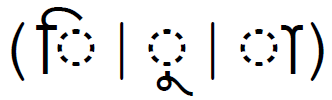
\includegraphics[height=1.2em]{\imgpath/banglaunicode.png} \z

If the converter needed to produce code for a different parsing engine, very little of the above code would need to change. In the case of the Xerox transducer (\texttt{xfst}), the only change would be to replace the parentheses with square brackets.

The code generator in (4) is simple, but some parts of the SFST code generator are comparatively complex, particularly the parts needed to handle morphosyntactic feature checking. The reason for the complexity is the fact that finite state transducers tend to treat the symbols for such features and their values as funny kinds of phonological characters, which have to be ignored in some circumstances, but paid attention to in others. It seems likely that future parsing engines will have special machinery for such features, which will considerably reduce the complexity of the converter. Even at present, though, the special machinery in the converter is hidden from the user, who need only worry about the higher level linguistic formalism.

While defining a formal grammar, and choosing a target parsing engine, allows us to straightforwardly define the converter code for the grammar in a language-independent way, dictionaries are a different matter. The target for dictionary converter code is defined by the parsing engine, but unless a dictionary is already in a standard format, converting the dictionary entry into that form must be done differently for each dictionary. Even when the dictionary uses a standard format (such as the ISO Lexical Markup Framework, ISO/TC 37/SC 4 2008), dictionaries of different languages may represent such things as inflection classes or stem allomorphy classes differently. As mentioned in the text, in some cases such classes may be represented only implicitly, by listing certain irregular forms; the morphosyntactic properties of these irregular forms must then be inferred. It may also be necessary to remove affixes from citation forms or irregular forms to obtain the stem. Fortunately, the structure of dictionaries--at least the parts that are needed for morphological parsers--is not as complex as grammars. In particular, senses and glosses, example sentences, and phrasal entries or phrasal sub-entries, can all be ignored.

\nocite{Knuth1999}
 
% Email for author: mmaxwell@casl.umd.edu
